\subsection{Spent Nuclear Fuel Simulations}
\label{sec:snfsim}

\begin{figure}[H]
  \centering
  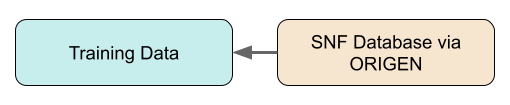
\includegraphics[width=0.7\linewidth]{./chapters/method/methodology1.png}
  \caption{First portion of the flowchart from Figure \ref{fig:method} being 
           described in this section.}
\end{figure}

Of interest to an entity trying to create a weapon is partially irradiated fuel
if they have plutonium separations capabilities or any radioactive substance in
the case of a dirty bomb. Thus, this work focuses on \gls{SNF} from commercial
power reactors. Ideally, a large enough database of \gls{SNF} nuclide assays
would be able to be used for this work. Since that does not exist, the 
database will be simulated via \gls{ORIGEN-ARP} \cite{origen, origenarp}.  

\subsubsection{Training Set Labels}
\label{sec:snflbls}

The design of the training set is dependent on a number of factors.  First, it
must have a sufficient number of burnup sets and time since irradiation steps
to provide robust prediction. This is decided upon by maximizing the steps for
both parameters, while balancing the computational limitations of a large
training set. Through previous experience, an approximate upper limit would be
somewhere around $1e6$ database entries for the specific calculations being
done in this work.

Secondly, the training set must represent what exists in the real world. This
was accomplished by studying the spread of parameters in the \gls{SFCOMPO}
database.  To ensure this, a variety of reactor types and assembly designs were
included, listed in Table \ref{tbl:rxtrtype}. Table \ref{tbl:rxtrparam} lists
the rest of the simulation inputs. These include not only the labels of
prediction interest, \gls{U235} enrichment, burnup, and time since irradiation,
but also other important simulation input parameters such as the reactor power
density and the moderator density.  (Water is both the moderator and coolant in
all simulated reactor types.)

\begin{table}[!h]
  \centering
  \begin{subtable}{\linewidth}
    \centering
    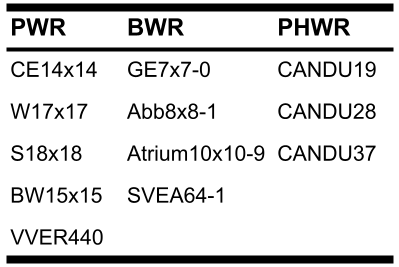
\includegraphics[width=0.55\linewidth]{./chapters/method/trainset4_Orxtrs.png}
    \caption{\gls{ORIGEN} designations for reactor technologies and fuel assembly design.}
    \label{tbl:rxtrtype}
    \vspace*{5mm}
  \end{subtable}
  \begin{subtable}{\linewidth}
    \centering
    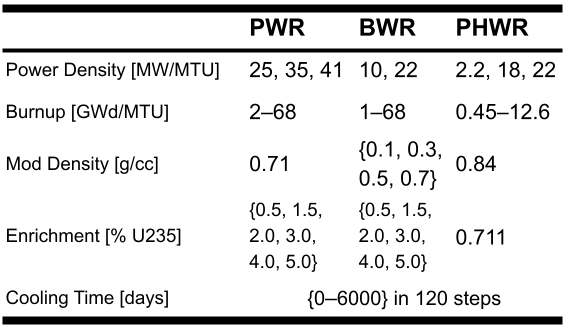
\includegraphics[width=0.8\linewidth]{./chapters/method/trainset4_inputs.png}
    \caption{Simulation parameters for \gls{ORIGEN} input files.}
    \label{tbl:rxtrparam}
  \end{subtable}%
  \caption{Training set database design using the \gls{SFCOMPO} database as guidance.}
  \label{tbl:train}
\end{table}

\todo[inline]{fix the figure, this is a placeholder}
\begin{figure}[!htb]
  \makebox[\textwidth][c]{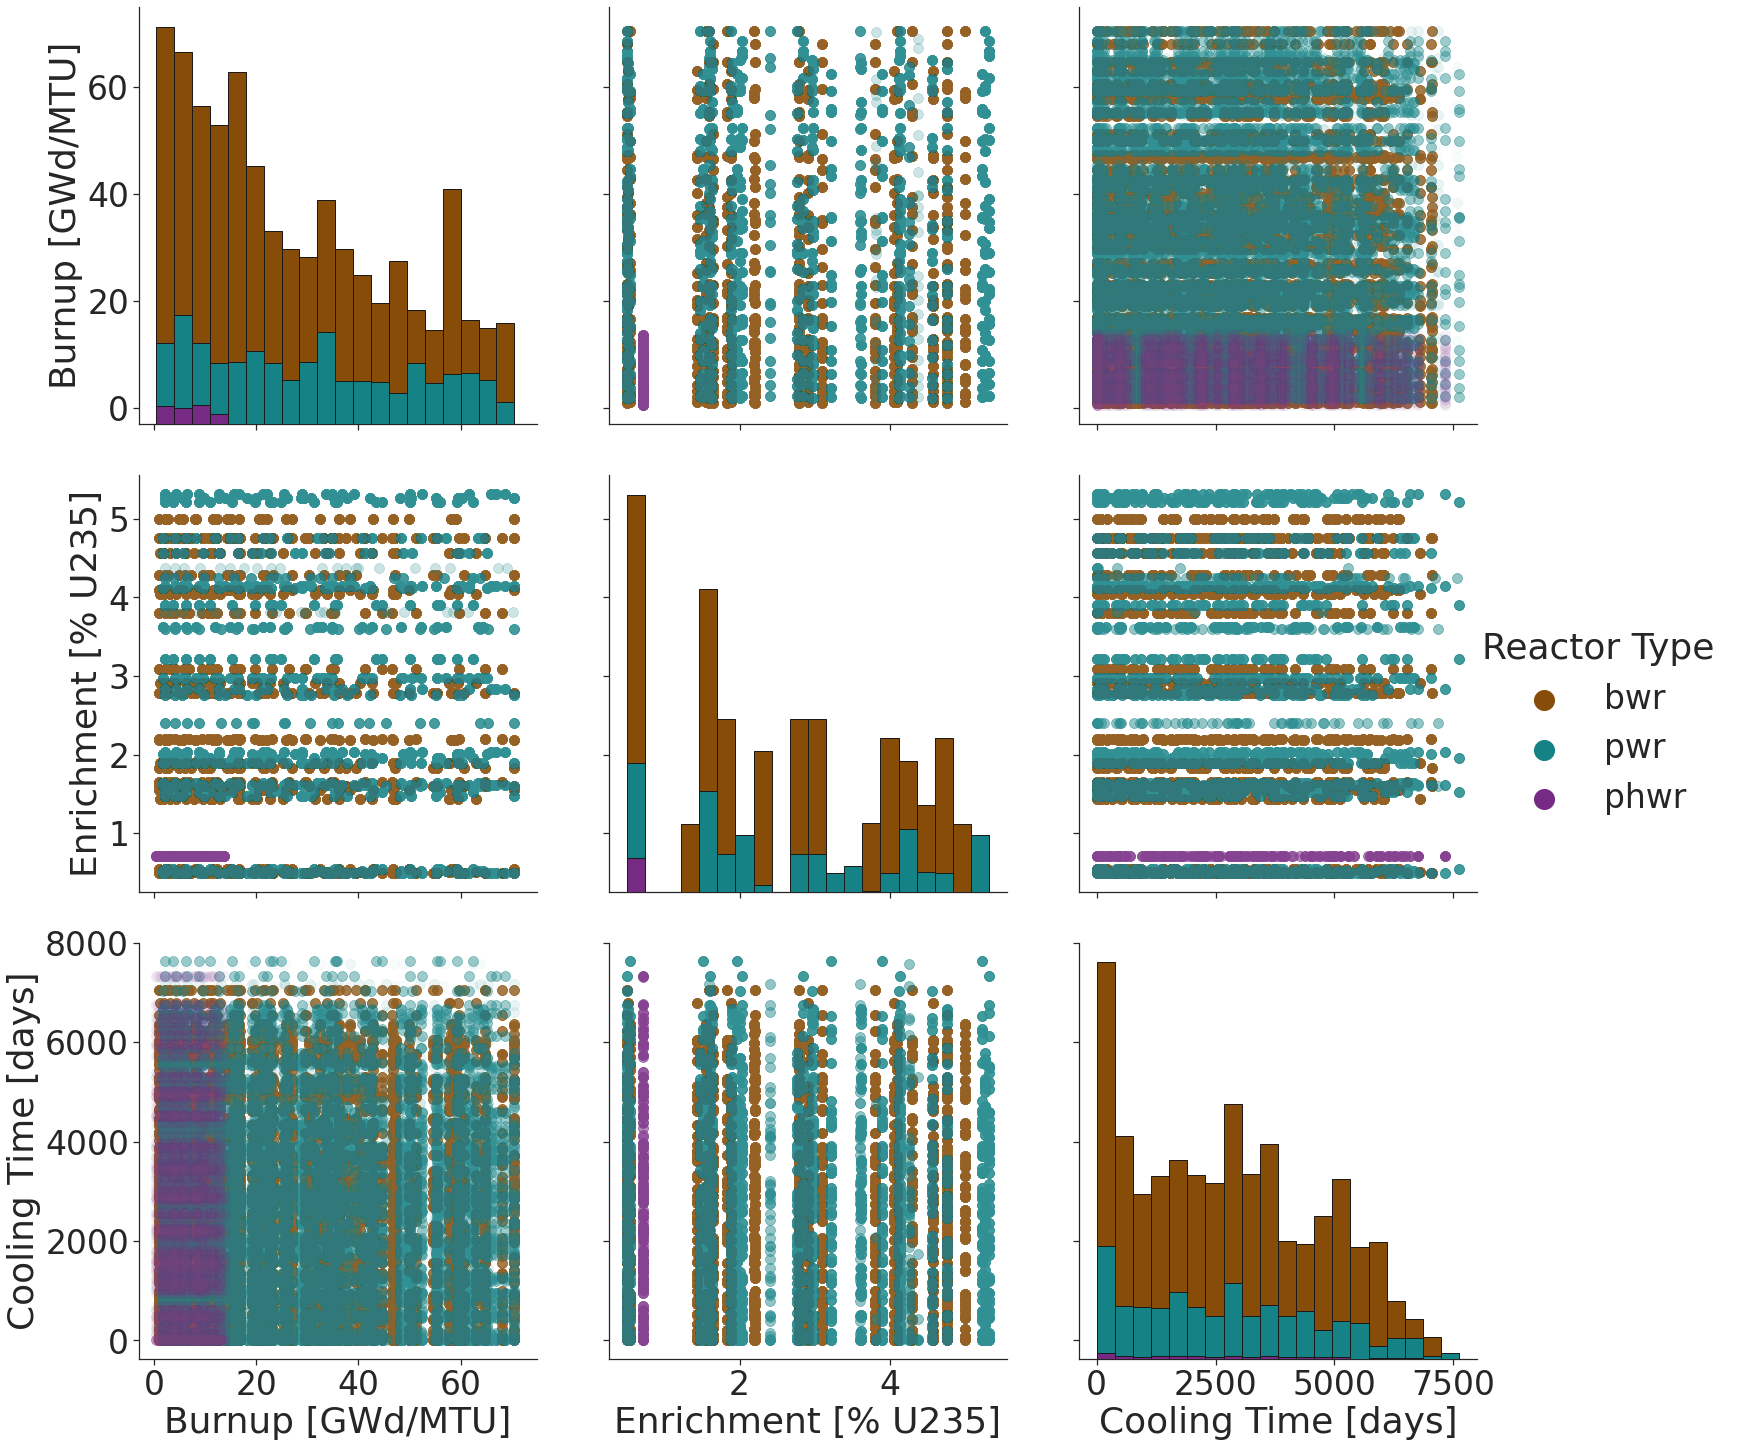
\includegraphics[width=\linewidth]{./chapters/method/histogram_scatter_trainset_viz.png}}
  \caption{A combination of histograms and scatter plots to visualize the 
           distribution of prediction labels in the training set.}
  \label{fig:trainhist}
\end{figure}

\todo[inline]{add section reference} The third factor influencing database
design is ensuring ideal \gls{ML} algorithm performance.  As mentioned in
Section X, many algorithms are developed with the assumption that the training
set will be \acrfull{i.i.d.}.  This is important so that the model does not
overvalue or overfit a certain area in the training space. With the training
set design, there are predetermined values for enrichment, burnup, and time
since irradiation.  While there are $21-28$ burnup steps (depending on the
reactor type) and 120 cooling time steps, there are only 6 values for
enrichment. This creates the risk that the algorithm will end up being unable
to generalize outside of those discrete values. Therefore, the burnup steps and
time steps are perturbed randomly in a range that is $\pm10\%$ and $\pm30\%$
from the originally defined values.  The enrichment also gets perturbed by
$\pm10\%$, and not more because the cross-section libraries in \gls{ORIGEN-ARP}
are pre-calculated for those enrichment values, so deviating too far from them
would result in inaccurate \gls{SNF} simulations. The power densities and
moderator densities were kept constant.  The resulting training set is $5e5$.
Figure \ref{fig:trainhist} visualizes the somewhat even distrubition of the
burnup and cooling time parameters, and shows the lack of even distribution of
the enrichment parameter through a combination of scatter plots and
histograms.\todo[inline]{enter new trainset size} 

\subsubsection{Training Set Features}
\label{sec:snffeats}

Hi hello.

\begin{table}[!h]
  \centering
  \begin{subtable}{\linewidth}
    \centering
    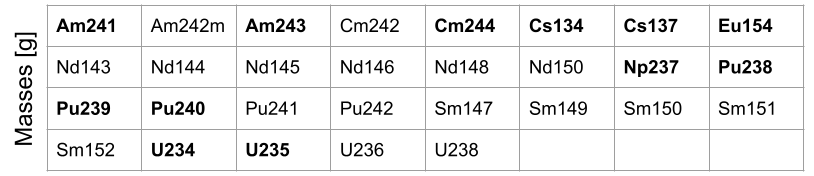
\includegraphics[width=\linewidth]{./chapters/method/nucmass_feats.png}
    \caption{Set of features saved for the first experiment. The bold nuclide
             masses overlap with the nuclides in \ref{tbl:nucacts}.}
    \label{tbl:nucmass}
    \vspace*{5mm}
  \end{subtable}
  \begin{subtable}{\linewidth}
    \centering
    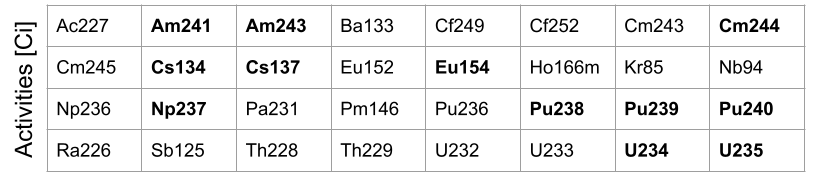
\includegraphics[width=\linewidth]{./chapters/method/nucacts_feats.png}
    \caption{Set of features saved for the second experiment. The bold nuclide
             activities overlap with the nuclides in \ref{tbl:nucmass}.}
    \label{tbl:nucacts}
  \end{subtable}%
  \caption{Two sets of features saved from the same simulation inputs for the 
           two main experiments in this work.}
  \label{tbl:nucfeats}
\end{table}

\subsection{Information Reduction}
\label{sec:inforeduc}

\begin{figure}[H]
  \centering
  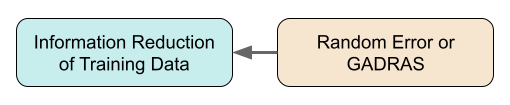
\includegraphics[width=0.7\linewidth]{./chapters/method/methodology2.png}
  \caption{Second portion of the flowchart from Figure \ref{fig:method} being 
           described in this section.}
\end{figure}

Since the overall goal of this project is to determine how much information to
what quality is needed to train an \gls{ML} model, there will be an
information reduction manipulation applied to the training data set. This study
evaluates the impact of randomly introduced error on the ability of the
algorithms to correctly predict the burnup. 

The three algorithms will be evaluated with error applied to each nuclide
vector in the training set.  A maximum error ranging from $0 - 10\%$ is chosen
for each round of training, and a random error within the range of $[1-E_{max},
1+E_{max}]$ is applied to each component of the nuclide vector.

However, error in a nuclide vector is not random, in fact it is systematic and
dependent on a number of known sources of uncertainty. The next study will
introduce error by limiting the nuclides to only those that can be measured
with a gamma spectrometer. Although this is initially done using the
availability of gamma energies in \gls{ORIGEN}, \gls{GADRAS} can provide more
\gls{DRF}s to further reduce information given to the algorithm.

Next, this work will expand upon the previous work.  The first future step is a
different information reduction technique using gamma energies from \gls{SNF}
nuclide recipes.  Following this, one could apply a \gls{DRF} that calculates
various spectra based on the types of gamma detectors available to the
forensics community 

